\section{Random binning features}

\begin{frame}
    \frametitle{Random Binning features}
    \textbf{Objective}:
    \begin{equation}
        k(\mathbf{x},\mathbf{y}) = \langle \phi(\mathbf{x}), \phi(\mathbf{y}) \rangle \approx z(\mathbf{x})^\prime z(\mathbf{y}). 
      \end{equation}
    \textbf{Algorithm description}
    \begin{itemize}
        \item  Partition the input space using randomly shifted grids at randomly chosen
        resolutions.
        \item Assigns to an input point a binary bit string that corresponds to the bins in which it
        falls.
        \item This mapping is well-suited
        for kernels that depend only on the $L_1$ distance between pairs of points. 
        \item The probability of two points of being in the same bin is proportional to $k(x,y)$.
        \item Finally $z(x)$ is a binary encoding of the bin where $x$ falls.
    \end{itemize}
\end{frame}

\begin{frame}
    \frametitle{Random Binning features: Graphical explanation}
% imgs/06_Random_features/random_binning_features.png
\begin{figure}[t]
    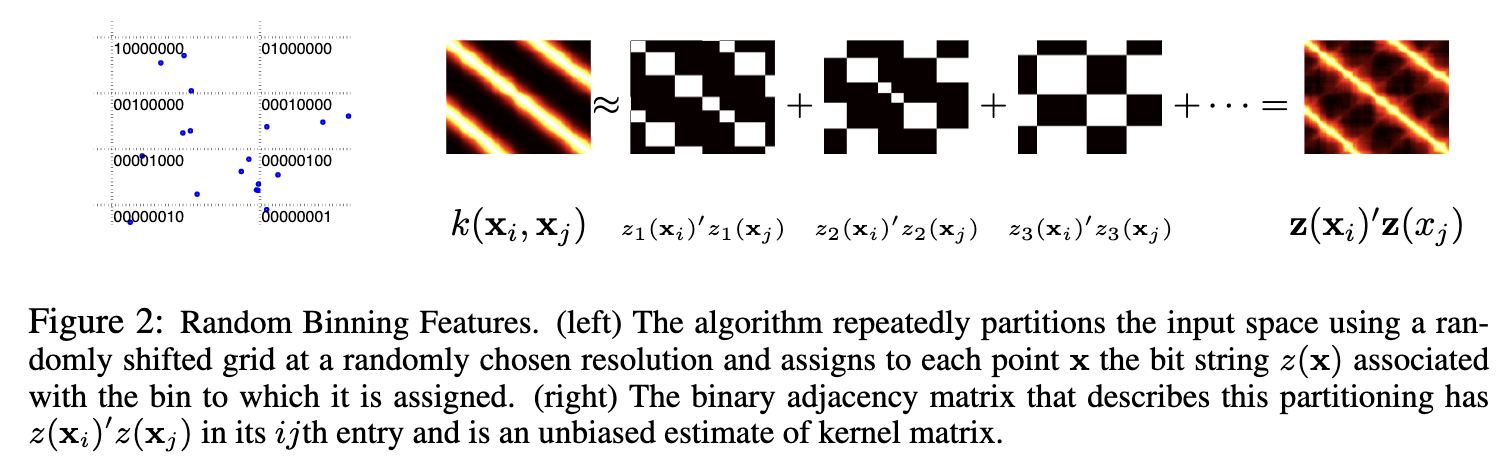
\includegraphics[width=\textwidth]{06_Random_features/random_binning_features.png}
    \centering
\end{figure}
    \begin{equation}
        z(x) = \sqrt{\frac{1}{P}}
        \left[
            z_1(x), \cdots, z_p(x)
        \right]^T
    \end{equation}
\end{frame}

\begin{frame}[fragile]
    \frametitle{Sklearnt aproximation: KBinsDiscretizer }
    
\begin{lstlisting}[style=PythonStyle]
    class sklearn.preprocessing.KBinsDiscretizer(
        n_bins=5, *, 
        encode='onehot', 
        strategy='quantile', 
        dtype=None, 
        subsample='warn',
        random_state=None)
\end{lstlisting}
Parameters:\footnote{
        Source: \url{https://scikit-learn.org/stable/modules/generated/sklearn.preprocessing.KBinsDiscretizer.html}
    }

\begin{itemize}
    \item \textbf{n\_bins}: The number of bins to produce.
    \item \textbf{encode}: \{‘onehot’, ‘onehot-dense’, ‘ordinal’\}.
    \item \textbf{strategy} \{‘uniform’, ‘quantile’, ‘kmeans’\}, default=’quantile’
    Strategy used to define the widths of the bins.
\end{itemize}
\end{frame}

\begin{frame}[fragile]
    \frametitle{How to use Random Binning Features}

\begin{lstlisting}[style=PythonStyle]
    >>> from sklearn.preprocessing import KBinsDiscretizer
    >>> X = [[0,100],[0,1],[1,0],[1,1],
    [2,2],[-1,1],[-1,1]]
    >>> est = KBinsDiscretizer(n_bins=3, encode='ordinal', strategy='uniform')
    >>> est.fit(X)
    KBinsDiscretizer(...)
    >>> Xt = est.transform(X)
    >>> Xt  
    array([[1., 2.],
    [1., 0.],
    [2., 0.],
    [2., 0.],
    [2., 0.],
    [0., 0.],
    [0., 0.]])
\end{lstlisting}

\end{frame}

\begin{frame}
    \frametitle{Sklearnt's KBinsDiscretizer is not the same that Random Binning Features}

    \begin{itemize}
        \item Deterministic.
        \item Feature by feature (do no transform the data).
    \end{itemize}
    \begin{table}[ht]
        \centering
        \caption{Input parameters for KBinsDiscretizer and the Random Binning Features algorithm}
        \label{tab:params}
        \begin{tabular}{c|c}
            \textbf{KBinsDiscretizer} & \textbf{Random Binning Features algorithm} \\
            \hline
            n\_bins & The output size $P$ \\
            encode &  A kernel function\\
            strategy &  \\
    
        \end{tabular}
    \end{table}  
\end{frame}

\begin{frame}
    \frametitle{Related works}

    \cite{exampleRandomBinning}
    \url{https://github.com/qw3rtman/random-feature-maps}
    \begin{itemize}
        \item Fast Random Kernelized Features: Support Vector Machine Classification for High-Dimensional IDC Dataset (2018), 
        \item First K-means,
        \item then random Features
        \item finally linear SVM classification. 
    \end{itemize}
    

\end{frame}

\begin{frame}
    \frametitle{Random Binning Features algorithm}

    \textbf{Input}
     \begin{itemize}
       % \item A point $x \in \R^d$.
        \item A kernel function $k(x,y) = k(x-y) =  \prod_{m=1}^d k_m(|x^m - y^m|)$, so that $p_m(h) \equiv h k_m''(h)$ is a probability distribution on $h \geq 0$.
    \end{itemize}
    
      
    \textbf{Algorithm} For $p \in \{1,\ldots, P\}$
    \begin{enumerate}
        \item  Draw grid parameters $h, u \in \mathbb{R}^d$ with the pitch $h^m \sim p_m$, and shift $u^m$ from the uniform distribution on $[0, h^m]$.
         \item Let $z$ return the coordinate of the bin containing $x$ as a binary indicator vector 
         $$
         z_p(x) \equiv 
         \text{hash}
         \left(
            \left\lfloor 
                \frac{x^1 - u^1}{h^1} 
            \right\rfloor,
             \dots, 
             \left\lfloor
                \frac{x^d - u^d}{h^d} 
            \right\rfloor
         \right).
         $$ 
    \end{enumerate}
    \textbf{Return}: A randomized feature map $z(x)$ so that $z(x)^Tz(y) \approx k(x-y)$.

\end{frame}

\begin{frame}
    \frametitle{kernel restrictions and how to compute $p$}

    \begin{lemma}
        \label{eq:lema1}
        Suppose a function $k(h): \mathbb{R} \rightarrow \mathbb{R}$ is twice differentiable and has the form
        \begin{equation}
            k(x) = \int_{\mathbb{R}} p(h) \max \left(0, 1- \frac{x}{h}\right) dh.
        \end{equation}
        Then $p(h) = h k''(h)$.
    \end{lemma}
    \pause
 \textbf{Proof}
 \begin{align}
    k(x) &= 
    \int_{\mathbb{R}} p(x) \max \left(0, 1- \frac{x}{h}\right) dh
    \\ 
    & = 
    % cero
    \int_{0}^x p(x) 0 dx
    + 
    \int_{x}^\infty
        p(x)
        \left(1- \frac{x}{h}\right) 
        d x
    \\
    &=
    \int_{x}^\infty
        p(h)
        dh
    -
    \int_{x}^\infty
        \frac{p(h) x}{h}
        d h. 
\end{align}
\end{frame}
\begin{frame}
    \frametitle{Proof}
    The Leibniz rule for derivatives formula:
   \begin{equation}
    \frac{d}{dx}\int_{a(x)}^{b(x)}f(x,t)dt=f(x,b(x))\frac{d}{dx}b(x)-f(x,a(x))\frac{d}{dx}a(x)+\int_{a(x)}^{b(x)}\frac{\partial}{\partial x}f(x,t)dt
   \end{equation}
    Hence
\begin{equation}
   k'(x)
   = 
   - p(x)
   - 
   \left[
    \int_{x}^\infty
            \frac{p(x)}{x}
            d x
    -
    x \frac{p(x)}{x}
   \right] 
   = - \int_{x}^\infty
   \frac{p(x)}{x}
   d x.
\end{equation}

    Applying a
    the Fundamental theorem of calculus: 

\begin{equation}
    k''(x)
    = 
    \frac{P(x)}{x}. 
\end{equation}

\end{frame}

\begin{frame}
    \frametitle{$K$ restriction}
    \begin{itemize}
        \item Twice differentiable,
        \item convex. 
    \end{itemize}

\end{frame}

\begin{frame}
    \frametitle{Math formulation }
    \begin{align}
        k_{hat}(x, y; h)
        & = 
        \max 
        \left(
        0,
        1 - \frac{|x-y|}{h}
        \right)  
        \\
        & = P\left[
        z(x)^T z(y) = 1 | h
    \right]
    \\
        & =
        E\left[
        z(x)^T z(y) = 1 | h
    \right]
    \end{align}

    By uniform $u \in U([0,h])$
    

\end{frame}

\begin{frame}
    \frametitle{Claim}
\begin{theorem}
        Let $M$ be a compact subset of $\mathbb{R}^d$ with diameter $\text{diam}(M)$. Let $\alpha = \mathbb{E}[1/delta]$ and let $L_k$ denote the Lipschitz constant of $k$ with respect to the $L_1$ norm. With $z$ as above, we have:
        \begin{equation}
            P \left[
                \sup_{x,y \in M} |z(x)^T z(y) - k(y,x)|
                \geq \varepsilon
            \right]
            \geq
            1 - 36 d P \alpha
            \text{ diam}(M)
            \exp\left(
                \frac{
                    - 
                    \left( 
                        \frac{P \epsilon^2}{8}
                        +
                        \ln \frac{\epsilon}{L_k}
                    \right)
                }{d +1 }
            \right)
        \end{equation}
    \end{theorem}

\end{frame}


\begin{frame}
    \frametitle{Next week}

    \begin{enumerate}
        \item “Nystroem Method vs Random Fourier Features: A Theoretical and Empirical Comparison”, Advances in Neural Information Processing Systems 2012
        \item Random features for kernel approximation: A survey on algorithms, theory, and beyond
        \item Williams, C.K.I. and Seeger, M. “Using the Nystroem method to speed up kernel machines”, Advances in neural information processing systems 2001
        T. Yang, Y. Li, M. Mahdavi, R. Jin and Z. Zhou 
        \item \url{https://proceedings.neurips.cc/paper_files/paper/2008/file/0efe32849d230d7f53049ddc4a4b0c60-Paper.pdf}
        \item Randomness in neural networks: an overview
        \item Fast and scalable polynomial kernels via explicit feature maps
        \item On the error of random Fourier features
        \item A survey on large-scale machine learning
        \item Sharp analysis of low-rank kernel matrix approximations
    \end{enumerate}

\end{frame}

\begin{frame}
    \frametitle{<title>}

    Para guardar código: 
    \url{https://scikit-learn.org/stable/model_persistence.html}
    Para sacar los modelos: 

    \url{https://www.csie.ntu.edu.tw/~cjlin/libsvmtools/datasets/}

\end{frame}
